%% ============================================================================
\section{Lecture 10: The Chandrasekhar Mass, Sound Waves, and Water Waves}
\label{sec:lec10}
%% ============================================================================
\date{18/06/2026}

\begin{center}
    \textit{Lecture date: 18/06/2026}
\end{center}

This lecture executes the Chandrasekhar-mass calculation set up at the end of
Lecture~9 and then applies the equipartition principle twice more: first to
derive the speed of sound from thermodynamics, and second to derive the
dispersion relations of both shallow and deep water waves. The unifying thread
is the same two-step recipe: (1) identify the two energy reservoirs in a wave or
bound system, (2) equate them and solve for the unknown frequency or mass.

%%----------------------------------------------------------------------------
\subsection{White Dwarf Mass--Radius Relation}
\label{sec:lec10:wd-setup}
%%----------------------------------------------------------------------------

\subsubsection*{Physical Motivation}
A white dwarf is a dead stellar core supported against gravitational collapse
not by thermal pressure (nuclear burning has ceased) but by the \emph{quantum}
pressure of degenerate electrons. The Pauli exclusion principle forbids two
electrons from occupying the same quantum state; when the star is compressed,
electrons are forced into ever higher momentum states, and the resulting
pressure resists further collapse. No temperature is required: this is
\emph{zero-temperature} quantum pressure.

We apply equipartition: gravitational binding energy $\sim |E_{\rm grav}|$ is
balanced by the total kinetic energy of the degenerate electrons $E_e$.

\subsubsection*{Electron Count and Number Density}

Let the white dwarf have total mass $M$ and radius $R$, and let its composition
be characterised by the mass number $A$ and atomic number $Z$ of the dominant
species (e.g.\ carbon-12 has $A=12$, $Z=6$). Define the
\emph{electrons-per-baryon} fraction
\begin{equation}
    \beta \equiv \frac{Z}{A}.
    \label{eq:lec10:beta}
\end{equation}
(For helium $\beta=1/2$; for carbon/oxygen $\beta=1/2$; $\beta=1$ only for
hydrogen.) The total number of nuclei is $N_{\rm nuc} = M/(Am_p)$, and since
the star is electrically neutral, the total electron count is
\begin{equation}
    \boxed{
    N_e = Z N_{\rm nuc} = \beta\,\frac{M}{m_p}.
    }
    \label{eq:lec10:Ne}
\end{equation}
\textit{Significance:} $N_e$ is fully determined by the mass and composition; the
electron fraction $\beta$ is a material constant of order $1/2$ for most white
dwarf compositions.

The mean electron number density is
\begin{equation}
    n_e = \frac{N_e}{V} = \frac{N_e}{\tfrac{4}{3}\pi R^3}
    \sim \frac{\beta M}{m_p R^3}.
    \label{eq:lec10:ne}
\end{equation}
(The exact factor $3/(4\pi)$ is an order-unity number, dropped throughout.)

\subsubsection*{Fermi Momentum from the Uncertainty Principle}

Each electron is confined to a volume $n_e^{-1}$ per particle, so its
positional uncertainty is $\Delta x \sim n_e^{-1/3}$. The uncertainty principle
then gives a minimum momentum:
\begin{equation}
    p_F \sim \frac{\hbar}{\Delta x} = \hbar\,n_e^{1/3}.
    \label{eq:lec10:pF}
\end{equation}
This is the \emph{Fermi momentum}: in a fully degenerate system all states up to
$p_F$ are filled and all states above are empty. The uncertainty principle
estimate reproduces the exact $p_F = \hbar(3\pi^2 n_e)^{1/3}$ up to an
order-unity factor.

\nt{Pitfall: the uncertainty principle gives a \emph{minimum} momentum, which is
also the \emph{typical} momentum in a degenerate zero-temperature gas — because
every electron is pushed to fill its allotted phase-space cell as compactly as
possible. In a classical gas the typical momentum is the thermal momentum
$\sqrt{2m_e k_B T}$, which is unrelated to density. Never confuse the two
regimes.}

%%----------------------------------------------------------------------------
\subsection{Non-Relativistic White Dwarf: $R \propto M^{-1/3}$}
\label{sec:lec10:wd-nr}
%%----------------------------------------------------------------------------

\subsubsection*{Mathematical Setup}

When $p_F \ll m_e c$ the electrons are non-relativistic. The kinetic energy per
electron is $\varepsilon_e = p_F^2/(2m_e)$, and the total electron kinetic
energy is
\begin{equation}
    E_e = N_e\,\varepsilon_e
    = N_e\,\frac{\hbar^2 n_e^{2/3}}{2m_e}
    = \frac{\hbar^2 N_e}{2m_e}\left(\frac{N_e}{R^3}\right)^{2/3}
    = \frac{\hbar^2 N_e^{5/3}}{2m_e R^2}.
    \label{eq:lec10:Ee-nr}
\end{equation}
The gravitational binding energy is
\begin{equation}
    |E_{\rm grav}| \sim \frac{G M^2}{R}.
    \label{eq:lec10:Egrav}
\end{equation}
\textit{Virial theorem reminder:} for gravity ($n=-1$), $\langle T\rangle =
-\tfrac{1}{2}\langle V\rangle$, so the kinetic energy \emph{equals half} the
magnitude of the potential energy in equilibrium. We absorb this factor of 2
into the order-of-magnitude symbol.

Setting $E_e \sim |E_{\rm grav}|$:
\begin{equation}
    \frac{\hbar^2 N_e^{5/3}}{2m_e R^2} \sim \frac{GM^2}{R}.
    \label{eq:lec10:equip-nr}
\end{equation}
Solving for $R$ and substituting $N_e = \beta M/m_p$:
\begin{equation}
    \boxed{
    R \sim \frac{\hbar^2 \beta^{5/3}}{m_e G\,m_p^{5/3}}\,M^{-1/3}.
    }
    \label{eq:lec10:R-nr}
\end{equation}
\textit{Significance:} In the non-relativistic regime, \emph{the more massive
the white dwarf, the smaller its radius} — a counter-intuitive result that
follows from $R^{-2}$ (confinement) dominating $R^{-1}$ (gravity). Adding mass
shrinks the star.

\ex[ex:lec10:wd-nr]{Worked Example: White Dwarf Radius for $M = M_\odot$}{
Take a carbon white dwarf ($\beta = 1/2$) with $M = M_\odot \approx 2\times10^{30}$\,kg.
Using SI units:
\[
    R \sim \frac{(1.055\times10^{-34})^2\,(0.5)^{5/3}}
           {(9.11\times10^{-31})(6.67\times10^{-11})(1.67\times10^{-27})^{5/3}}
    \times
    (2\times10^{30})^{-1/3}
\]
The numerical prefactor works out to $\sim 10^{9}$\,m\,$\times$\,kg$^{1/3}$,
and $M^{-1/3}\approx (2\times10^{30})^{-1/3}\approx 8\times10^{-11}$\,kg$^{-1/3}$, giving
\[
    R \sim \text{a few}\times 10^{6}\,\text{m} = \text{a few thousand km.}
\]
Astronomically observed white dwarfs have radii $R \sim 5000$\,km $\approx R_\oplus$
--- the estimate is correct.
}

%%----------------------------------------------------------------------------
\subsection{Relativistic Limit: The Chandrasekhar Mass}
\label{sec:lec10:chandrasekhar}
%%----------------------------------------------------------------------------

\subsubsection*{Physical Motivation}
As $M$ grows, $R$ decreases and $n_e$ rises as $n_e \propto M/R^3 \propto
M^2$. The Fermi momentum $p_F \propto n_e^{1/3} \propto M^{2/3}$ eventually
approaches $m_e c$, and the electrons become \emph{relativistic}. In the
extreme relativistic limit $p_F \gg m_e c$, the electron energy is $\varepsilon_e
= p_F c$ rather than $p_F^2/(2m_e)$. This change in the energy-momentum
relation has a dramatic consequence.

\subsubsection*{Derivation}

Replace $\varepsilon_e = p_F^2/(2m_e)$ with $\varepsilon_e = p_F c = \hbar c\,n_e^{1/3}$:
\begin{equation}
    E_e = N_e\,\varepsilon_e
    = N_e\,\hbar c\,n_e^{1/3}
    = \hbar c\,N_e \left(\frac{N_e}{R^3}\right)^{1/3}
    = \frac{\hbar c\,N_e^{4/3}}{R}.
    \label{eq:lec10:Ee-rel}
\end{equation}
Now set $E_e \sim |E_{\rm grav}|$:
\begin{equation}
    \frac{\hbar c\,N_e^{4/3}}{R} \sim \frac{GM^2}{R}.
    \label{eq:lec10:equip-rel}
\end{equation}
The radius $R$ cancels. This is the key fact: in the relativistic limit,
equipartition does \emph{not} determine $R$ --- it determines $M$. Substituting
$N_e = \beta M/m_p$:
\begin{equation}
    \hbar c\,\left(\frac{\beta M}{m_p}\right)^{4/3} \sim G M^2
    \quad\Longrightarrow\quad
    M^{2/3} \sim \frac{\hbar c\,\beta^{4/3}}{G\,m_p^{4/3}}.
    \label{eq:lec10:Mch-step}
\end{equation}
Raising both sides to the power $3/2$:

\thm[thm:lec10:chandrasekhar]{Chandrasekhar Mass}{
The maximum mass a white dwarf can have is
\begin{equation}
    \boxed{
    M_{\rm Ch} \sim \left(\frac{\hbar c}{G}\right)^{3/2}\frac{\beta^2}{m_p^2}
    = \beta^2\,m_p\left(\frac{\hbar c}{Gm_p^2}\right)^{3/2}.
    }
    \label{eq:lec10:Mch}
\end{equation}
Above this mass, no white dwarf equilibrium exists: gravity overwhelms quantum
pressure and the star collapses.
}

\textit{Significance:} $M_{\rm Ch}$ is set by fundamental constants alone ---
no free parameters. The appearance of $\hbar c/G$ combines gravity with quantum
mechanics and special relativity; it is the energy scale at which gravitational
binding energy of a proton pair equals the Compton energy of an electron.

\subsubsection*{Physical Interpretation via $\alpha_G$}

Define the gravitational analogue of the fine-structure constant,
\begin{equation}
    \alpha_G \equiv \frac{Gm_p^2}{\hbar c}
    \approx \frac{(6.67\times10^{-11})(1.67\times10^{-27})^2}
                 {(1.055\times10^{-34})(3\times10^8)}
    \approx 5.9\times10^{-39}.
    \label{eq:lec10:alphaG}
\end{equation}
Then
\begin{equation}
    \boxed{
    M_{\rm Ch} \sim \frac{\beta^2\,m_p}{\alpha_G^{3/2}}.
    }
    \label{eq:lec10:Mch-alphaG}
\end{equation}
\textit{Significance:} $M_{\rm Ch}$ is enormous compared to the proton mass
\emph{precisely because gravity is so weak} ($\alpha_G \ll 1$). The white
dwarf radius is
\begin{equation}
    R_{\rm WD} \sim \frac{\lambda_e}{\alpha_G^{1/2}},
    \qquad
    \lambda_e \equiv \frac{\hbar}{m_e c} \approx 3.86\times10^{-13}\,\text{m}
    \label{eq:lec10:RWD}
\end{equation}
(the electron Compton wavelength), which is macroscopic ($\sim 10^{6}$\,km) only
because $\alpha_G^{1/2}$ is tiny.

\ex[ex:lec10:Mch-numeric]{Worked Example: Numerical Estimate of $M_{\rm Ch}$}{
For $\beta = 1/2$ (carbon white dwarf):
\[
    \alpha_G^{3/2} \approx (5.9\times10^{-39})^{3/2}
    \approx (5.9)^{3/2}\times10^{-58.5}
    \approx 14.3\times 3.2\times10^{-59}
    \approx 4.6\times10^{-58}.
\]
\[
    M_{\rm Ch} \sim \frac{(1/2)^2 \times 1.67\times10^{-27}}{4.6\times10^{-58}}
    \approx \frac{4.2\times10^{-28}}{4.6\times10^{-58}}
    \approx 9\times10^{29}\,\text{kg}
    \approx 0.45\,M_\odot.
\]
The exact Chandrasekhar mass is $1.4\,M_\odot$; the order-of-magnitude estimate
is off by a factor of $\sim 3$, which comes from the missing numerical
prefactor in the Fermi energy (integrating the Fermi--Dirac distribution gives
an exact coefficient of $(9\pi/4)^{2/3}/5 \approx 0.6$ instead of 1). The
order-of-magnitude result is correct.
}

\nt{Pitfall: the Chandrasekhar limit is often quoted as $\approx 1.4\,M_\odot$
for a carbon/oxygen white dwarf ($\beta = 1/2$). Do not confuse $M_{\rm Ch}
\propto \beta^2$: a hydrogen white dwarf ($\beta=1$) would have $M_{\rm Ch}
\approx 4\times 1.4\,M_\odot$ --- but hydrogen white dwarfs are not found
in nature because the star burns its hydrogen before the core becomes degenerate.}

\subsubsection*{Method: Estimating Quantum Equilibrium Masses}
\begin{enumerate}
    \item Identify the quantum pressure source (degenerate electrons, neutrons,
    etc.) and write its energy $E_{\rm kin}$ as a function of $N$, $R$, and
    fundamental constants.
    \item Write the gravitational energy $|E_{\rm grav}| \sim GM^2/R$.
    \item Set $E_{\rm kin} \sim |E_{\rm grav}|$ and solve:
    \begin{itemize}
        \item Non-relativistic ($\varepsilon \propto p^2$): $E_{\rm kin}\propto
        R^{-2}$ and $E_{\rm grav}\propto R^{-1}$ --- there is \emph{always} a
        stable equilibrium radius for any $M$, and $R\propto M^{-1/3}$.
        \item Ultra-relativistic ($\varepsilon\propto p$): $E_{\rm kin}\propto
        R^{-1}$ and $E_{\rm grav}\propto R^{-1}$ --- both scale the same way.
        Equilibrium exists only at one special mass $M_{\rm Ch}$; for $M>M_{\rm Ch}$
        there is no equilibrium.
    \end{itemize}
    \item Check the self-consistency of the approximation: was the non-relativistic
    or relativistic limit the right one?
\end{enumerate}

\subsubsection*{The $R$--$M$ Curve}

\begin{figure}[ht]
    \centering
    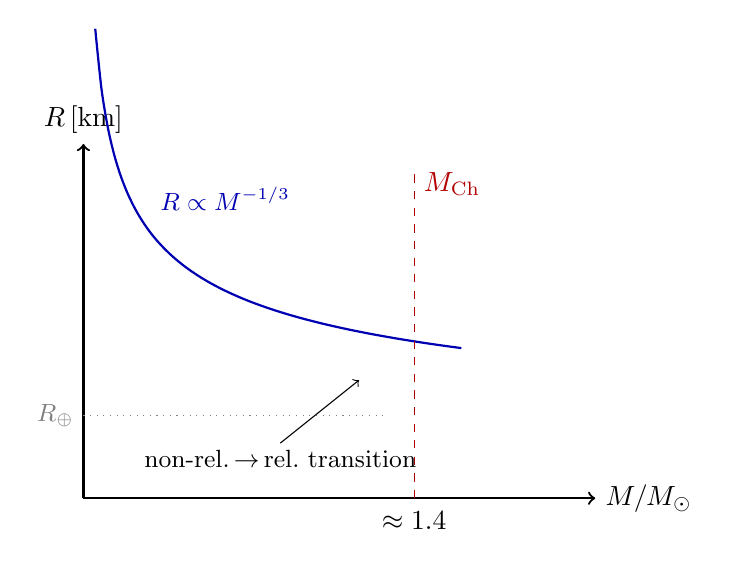
\begin{tikzpicture}[scale=1.0]
        \draw[thick,->] (0,0) -- (6.5,0) node[right] {$M/M_\odot$};
        \draw[thick,->] (0,0) -- (0,4.5) node[above] {$R$\,[km]};
        % non-relativistic branch R ~ M^{-1/3}
        \draw[thick,blue!70!black,domain=0.15:4.8,smooth,samples=60]
            plot (\x, {3.2/\x^0.33});
        % asymptotic Chandrasekhar mass
        \draw[dashed,red!70!black] (4.2,0) -- (4.2,4.2)
            node[pos=0.95,right] {$M_{\rm Ch}$};
        \draw (4.2,-0.05) node[below] {$\approx 1.4$};
        % labels
        \node[blue!70!black] at (1.8,3.8)
            {\small $R\propto M^{-1/3}$};
        \node at (2.5,0.5) {\small non-rel.\,$\to$\,rel.\ transition};
        \draw[->] (2.5,0.7) -- (3.5,1.5);
        % R_Earth
        \draw[dotted,gray] (0,1.05) node[left] {\small $R_\oplus$} -- (3.8,1.05);
    \end{tikzpicture}
    \caption{White dwarf mass--radius relation. In the non-relativistic limit
    $R\propto M^{-1/3}$ (blue curve). As $M\to M_{\rm Ch}$ the electrons
    become ultra-relativistic and the curve bends steeply toward $R\to0$;
    above $M_{\rm Ch}$ there is no equilibrium.}
    \label{fig:lec10:wd-rm}
\end{figure}

%%----------------------------------------------------------------------------
\subsection{Neutron Stars and the Oppenheimer--Volkoff--Tolman Limit}
\label{sec:lec10:neutron-stars}
%%----------------------------------------------------------------------------

\subsubsection*{Physical Motivation}
What happens when $M>M_{\rm Ch}$? The white dwarf collapses further. At
densities comparable to nuclear matter, it becomes energetically favourable for
protons and electrons to merge into neutrons via inverse beta decay:
$p^+ + e^- \to n + \nu_e$. The resulting object --- a \emph{neutron star} --- is
supported by \emph{neutron} degeneracy pressure rather than electron degeneracy
pressure. The same calculation applies with the substitution $m_e\to m_n$.

\subsubsection*{Critical Mass and Radius}

The maximum mass (Oppenheimer--Volkoff--Tolman or OVT mass) has the same
structure as Eq.~\eqref{eq:lec10:Mch} but with the neutrons playing both roles
(providing the pressure and the mass):
\begin{equation}
    \boxed{
    M_{\rm OVT} \sim m_p\,\alpha_G^{-3/2} \sim M_{\rm Ch}(\beta=1),
    }
    \label{eq:lec10:Movt}
\end{equation}
which is also $\sim 2\,M_\odot$ (the exact value depends on the poorly-known
nuclear equation of state at super-nuclear densities).

The characteristic radius scales as
\begin{equation}
    R_{\rm NS} \sim \frac{\hbar}{m_n c}\,\alpha_G^{-1/2}
    \approx \frac{m_e}{m_n}\,R_{\rm WD}
    \approx \frac{R_{\rm WD}}{1836}
    \sim \text{10 km}.
    \label{eq:lec10:Rns}
\end{equation}
\textit{Significance:} The neutron star is roughly 2000 times smaller than a white
dwarf of the same mass, compressed to a radius comparable to a city.

\nt{The equation of state of matter at densities above nuclear ($\rho\gtrsim
10^{17}\,\text{kg\,m}^{-3}$) is unknown: quarks may deconfine into a quark--gluon
plasma, and exotic hyperon matter may appear. For this reason, neutron star
structure cannot be solved as cleanly as white dwarf structure, and radius
measurements are used to constrain the nuclear equation of state. Ongoing NICER
X-ray timing observations are now placing firm constraints.}

%%----------------------------------------------------------------------------
\subsection{Sound Waves via Equipartition}
\label{sec:lec10:sound}
%%----------------------------------------------------------------------------

\subsubsection*{Physical Motivation}
An acoustic (sound) wave is a small-amplitude compressional wave in a fluid. As
it propagates, energy oscillates between two reservoirs:
\begin{itemize}
    \item \textbf{Kinetic energy}: the fluid elements move with velocity $v_1$.
    \item \textbf{Internal energy}: alternating compressions and rarefactions
    store energy as increased (decreased) density and pressure.
\end{itemize}
Equipartition guarantees that the time-averaged energies are equal (both are
quadratic in the wave amplitude). Equating them, and using the linearized
continuity equation to link $v_1$ and $\delta\rho$, yields the dispersion
relation.

\subsubsection*{Thermodynamic Setup: The Isentropic Condition}

A crucial input is the \emph{nature} of the perturbation. Sound waves are
isentropic (adiabatic): the compression and rarefaction happen much faster than
heat can diffuse between adjacent fluid elements. Formally, the entropy per
unit mass $s$ is constant along a fluid trajectory,
\begin{equation}
    \frac{Ds}{Dt} = 0,
    \label{eq:lec10:isentropic}
\end{equation}
which means we should evaluate energy derivatives at constant $s$ (equivalently,
at constant entropy per unit mass).

\subsubsection*{Internal Energy Perturbation from the First Law}

Let $\rho_0,\,S_0$ be the equilibrium density and entropy, and write
$\rho = \rho_0 + \delta\rho$ with $\delta\rho \ll \rho_0$. The internal energy
density $u_{\rm int} = \rho\varepsilon(\rho,s)$ (where $\varepsilon$ is the
specific internal energy) must be Taylor-expanded to second order to find the
wave energy:
\begin{equation}
    \rho\varepsilon
    =
    \rho_0\varepsilon_0
    +
    \left.\frac{\partial(\rho\varepsilon)}{\partial\rho}\right|_s\delta\rho
    +
    \frac{1}{2}\left.\frac{\partial^2(\rho\varepsilon)}{\partial\rho^2}\right|_s
    (\delta\rho)^2
    +\ldots
    \label{eq:lec10:uexpand}
\end{equation}

\paragraph{First derivative.}
The thermodynamic first law for a fluid element of specific volume
$v\equiv1/\rho$ is
\begin{equation}
    d\varepsilon = T\,ds - P\,dv = T\,ds + \frac{P}{\rho^2}\,d\rho.
    \label{eq:lec10:firstlaw}
\end{equation}
Therefore
\begin{align}
    d(\rho\varepsilon)
    &= \varepsilon\,d\rho + \rho\,d\varepsilon
    = \varepsilon\,d\rho + \rho\!\left(T\,ds + \frac{P}{\rho^2}\,d\rho\right)
    \notag\\
    &= \underbrace{\left(\varepsilon + \frac{P}{\rho}\right)}_{h}\,d\rho
      + \rho T\,ds,
    \label{eq:lec10:drhoeps}
\end{align}
where $h = \varepsilon + P/\rho$ is the specific enthalpy. At constant entropy
($ds=0$):
\begin{equation}
    \left.\frac{\partial(\rho\varepsilon)}{\partial\rho}\right|_s = h_0.
    \label{eq:lec10:d1}
\end{equation}

\paragraph{Second derivative.}
Differentiating $h$ with respect to $\rho$ at constant $s$:
\begin{align}
    \left.\frac{\partial h}{\partial\rho}\right|_s
    &=
    \left.\frac{\partial\varepsilon}{\partial\rho}\right|_s
    + \frac{1}{\rho}\left.\frac{\partial P}{\partial\rho}\right|_s
    - \frac{P}{\rho^2}
    \notag\\
    &=
    \underbrace{\frac{P}{\rho^2}}_{\text{from first law}}
    + \frac{c_s^2}{\rho}
    - \frac{P}{\rho^2}
    =
    \frac{c_s^2}{\rho_0},
    \label{eq:lec10:d2}
\end{align}
where we define the \emph{adiabatic sound speed}
\begin{equation}
    \boxed{
    c_s^2 \equiv \left.\frac{\partial P}{\partial\rho}\right|_s.
    }
    \label{eq:lec10:cs-def}
\end{equation}

\paragraph{Wave energy contribution.}
The linear term $h_0\,\delta\rho$ averages to zero over a complete wave cycle
because mass conservation requires $\langle\delta\rho\rangle = 0$. The
quadratic term gives the internal energy fluctuation per unit volume:
\begin{equation}
    \langle\delta u_{\rm int}\rangle
    = \frac{c_s^2}{2\rho_0}\langle(\delta\rho)^2\rangle.
    \label{eq:lec10:u-int-wave}
\end{equation}

\subsubsection*{Linking $\delta\rho$ and $v_1$ via Continuity}

The linearized continuity (mass-conservation) equation is
\begin{equation}
    \frac{\partial(\delta\rho)}{\partial t}
    + \rho_0\,\nabla\cdot\vb*{v}_1 = 0.
    \label{eq:lec10:continuity}
\end{equation}
For a plane wave $\delta\rho,\,v_1 \propto e^{i(kx-\omega t)}$ this becomes
\begin{equation}
    -i\omega\,\delta\rho + i k\,\rho_0\,v_1 = 0
    \quad\Longrightarrow\quad
    \delta\rho = \frac{k\rho_0}{\omega}\,v_1,
    \label{eq:lec10:continuity-plane}
\end{equation}
so $\langle(\delta\rho)^2\rangle = (k\rho_0/\omega)^2\langle v_1^2\rangle$.

\subsubsection*{Derivation of the Dispersion Relation}

The mean kinetic energy density is $\langle KE\rangle = \tfrac{1}{2}\rho_0\langle
v_1^2\rangle$. Setting $\langle KE\rangle = \langle\delta u_{\rm int}\rangle$:
\begin{align}
    \frac{1}{2}\rho_0\langle v_1^2\rangle
    &=
    \frac{c_s^2}{2\rho_0}\cdot\frac{k^2\rho_0^2}{\omega^2}\langle v_1^2\rangle
    \notag\\
    \rho_0 &= \frac{c_s^2 k^2\rho_0}{\omega^2}
    \notag\\
    \omega^2 &= c_s^2 k^2.
    \label{eq:lec10:sound-dispersion-derivation}
\end{align}

\thm[thm:lec10:sound]{Sound Wave Dispersion Relation}{
Acoustic waves in an isentropic fluid satisfy
\begin{equation}
    \boxed{
    \omega = c_s k,
    \qquad
    c_s = \sqrt{\left.\frac{\partial P}{\partial\rho}\right|_s}.
    }
    \label{eq:lec10:sound-dispersion}
\end{equation}
This is a non-dispersive relation: all frequencies travel at the same phase
velocity $c_s$, independent of $k$.
}

\textit{Significance:} Sound is non-dispersive precisely because the energy
equation is quadratic (harmonic) in both $v_1$ and $\delta\rho$, and equipartition
holds exactly. The adiabatic condition is physical: at the frequencies of audible
sound, molecules do not have time to exchange heat between compressed and
rarefied regions.

\ex[ex:lec10:sound-ideal-gas]{Worked Example: Sound Speed in an Ideal Gas}{
For an ideal gas undergoing an adiabatic process, $P = K\rho^\gamma$ (constant
entropy means $K = P_0/\rho_0^\gamma$ is fixed), so
\[
    \left.\frac{\partial P}{\partial\rho}\right|_s
    = K\gamma\rho^{\gamma-1}
    = \gamma\frac{P}{\rho}
    = \gamma\frac{k_B T}{\bar{m}},
\]
where $\bar{m}$ is the mean molecular mass. Thus
\[
    \boxed{c_s = \sqrt{\frac{\gamma k_B T}{\bar{m}}}}.
\]
For air ($\gamma=7/5$, $\bar{m}=29\,m_u$) at $T=293\,\text{K}$:
\[
    c_s = \sqrt{\frac{1.4\times 1.38\times10^{-23}\times293}{29\times1.66\times10^{-27}}}
    \approx 343\,\text{m/s}.
\]
This is the familiar speed of sound in air. Note: if we had used the
\emph{isothermal} derivative $(\partial P/\partial\rho)_T = k_BT/\bar{m}$ (Newton's
original mistake), we would get $c_s^{\rm Newton}=c_s/\sqrt{\gamma}\approx290$\,m/s
--- off by the factor $\sqrt{\gamma}$, first corrected by Laplace.
}

\nt{Pitfall: the isothermal vs.\ isentropic distinction matters:
$c_s^{\rm isen}/c_s^{\rm iso}=\sqrt{\gamma}\approx 1.18$ for air. Newton's
calculation of the speed of sound was 18\,\% too slow because he assumed
isothermal compressions. The correct (adiabatic) formula was given by Laplace.
Always use $(\partial P/\partial\rho)_s$ for sound.}

\subsubsection*{Method: Deriving Wave Dispersion via Equipartition}
\begin{enumerate}
    \item Identify the two energy reservoirs and write their densities to second
    order in the wave amplitude.
    \item Use a conservation law (here: mass continuity) to relate the two
    amplitudes for a monochromatic wave $e^{i(kx-\omega t)}$.
    \item Set the time-averaged densities equal and cancel the common
    amplitude squared.
    \item Read off $\omega(k)$.
\end{enumerate}
The key check: both energy densities must be quadratic in the amplitude; only
then does equipartition hold exactly and the amplitude cancels cleanly.

%%----------------------------------------------------------------------------
\subsection{Shallow Water Waves via Equipartition}
\label{sec:lec10:shallow-water}
%%----------------------------------------------------------------------------

\subsubsection*{Physical Motivation}
Gravity waves on the surface of water exchange kinetic energy (fluid motion)
with gravitational potential energy (surface displacement). Unlike sound, these
waves are \emph{not} compressional: the water is treated as incompressible
($\nabla\cdot\vb*{v}=0$), so there is no internal energy term. The depth $H$
(if finite) enters as a new length scale that constrains the fluid motion.

\begin{figure}[ht]
    \centering
    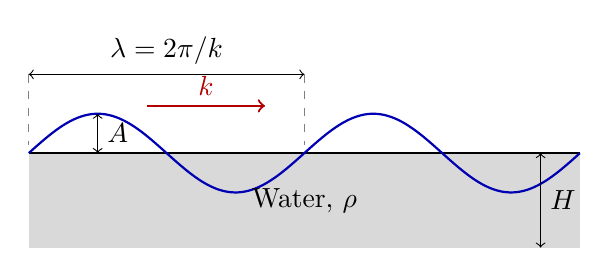
\begin{tikzpicture}[scale=1.0]
        % seafloor
        \fill[gray!30] (0,-1.2) rectangle (7,0);
        \draw[thick] (0,0) -- (7,0);
        % water surface (sinusoidal)
        \draw[thick,blue!70!black,domain=0:7,smooth,samples=80]
            plot (\x, {0.5*sin(deg(2*3.14159*\x/3.5))});
        % labels
        \draw[<->] (6.5,-1.2) -- (6.5,0) node[midway,right] {$H$};
        \draw[<->] (0.875,0) -- (0.875,0.5) node[midway,right] {$A$};
        \draw[<->] (0,1.0) -- (3.5,1.0) node[midway,above] {$\lambda=2\pi/k$};
        \draw[dashed,gray] (0,1.0) -- (0,0.1);
        \draw[dashed,gray] (3.5,1.0) -- (3.5,0.1);
        % wave vector
        \draw[->,thick,red!70!black] (1.5,0.6) -- (3.0,0.6)
            node[midway,above] {$k$};
        % depth label
        \node at (3.5,-0.6) {Water, $\rho$};
    \end{tikzpicture}
    \caption{Shallow water wave geometry. The amplitude $A\ll H$ is the surface
    displacement; $H$ is the water depth; $k=2\pi/\lambda$ is the wavenumber.}
    \label{fig:lec10:shallow-water}
\end{figure}

\subsubsection*{Potential Energy}

For a surface displacement $\eta = A\cos(kx-\omega t)$, the crest region
rises a height $A$ above the mean. The gravitational potential energy stored
per unit surface area is of order
\begin{equation}
    \langle PE\rangle/\text{area} \sim \rho g A^2.
    \label{eq:lec10:sw-pe}
\end{equation}
(The exact coefficient is $\tfrac{1}{2}$, from lifting mass $\rho A$ per unit
area by $A/2$, but order-of-magnitude estimates ignore the $\tfrac{1}{2}$.)

\subsubsection*{Kinetic Energy via Mass Conservation}

The key is to find the fluid velocity amplitude $v_1$. Over one half-period
$\pi/\omega$, the mass per unit width in a surface crest of height $A$ and
horizontal extent $k^{-1}$ must be transported horizontally to the adjacent
trough. The total mass per unit width is $\sim\rho A k^{-1}$; this must pass
through the water column of depth $H$. From the linearized continuity equation
(integrating from bottom to surface),
\begin{equation}
    \partial_t\eta + H\,\partial_x v_1 = 0
    \quad\Longrightarrow\quad
    -i\omega A + ikHv_1 = 0
    \quad\Longrightarrow\quad
    \boxed{v_1 = \frac{\omega A}{kH}.}
    \label{eq:lec10:sw-vel}
\end{equation}
The kinetic energy per unit area is
\begin{equation}
    \langle KE\rangle/\text{area}
    \sim \rho H v_1^2
    = \rho H\,\frac{\omega^2 A^2}{k^2 H^2}
    = \frac{\rho\omega^2 A^2}{k^2 H}.
    \label{eq:lec10:sw-ke}
\end{equation}

\subsubsection*{Equipartition}

Setting $\langle KE\rangle = \langle PE\rangle$ and cancelling $\rho A^2$:
\begin{equation}
    \frac{\omega^2}{k^2 H} \sim g
    \quad\Longrightarrow\quad
    \omega^2 = gk^2 H.
    \label{eq:lec10:sw-dispersion-deriv}
\end{equation}

\thm[thm:lec10:shallow-water]{Shallow Water Dispersion Relation}{
\begin{equation}
    \boxed{
    \omega^2 = gk^2 H,
    \qquad
    v_{\rm phase} = \frac{\omega}{k} = \sqrt{gH}.
    }
    \label{eq:lec10:shallow-water}
\end{equation}
The phase velocity is \emph{independent of wavenumber}: shallow water waves are
\textbf{non-dispersive}. All wavelengths travel at the same speed $\sqrt{gH}$.
}

\textit{Significance:} The depth $H$ plays the role of the restoring parameter.
When $kH\ll1$ (wavelength much larger than depth, i.e.\ the ``shallow'' condition),
this formula applies regardless of the wavelength.

%%----------------------------------------------------------------------------
\subsection{Deep Water Waves}
\label{sec:lec10:deep-water}
%%----------------------------------------------------------------------------

\subsubsection*{Physical Motivation}
For deep water ($kH\gg1$), the water column extends far below the surface; the
fluid velocity due to the wave decays exponentially with depth on a scale
$k^{-1}$ (the wavelength). The water far below ``does not know'' about the
surface wave. In this limit the effective depth is replaced by the only
remaining length scale, $H\to k^{-1}$:
\begin{equation}
    \omega^2 = gk^2\cdot k^{-1} = gk.
    \label{eq:lec10:dw-derivation}
\end{equation}

\thm[thm:lec10:deep-water]{Deep Water Dispersion Relation}{
\begin{equation}
    \boxed{
    \omega^2 = gk,
    \qquad
    v_{\rm phase} = \sqrt{\frac{g}{k}} = \sqrt{\frac{g\lambda}{2\pi}}.
    }
    \label{eq:lec10:deep-water}
\end{equation}
Deep water waves are \textbf{dispersive}: longer wavelengths travel faster. The
group velocity $v_g = d\omega/dk = \tfrac{1}{2}\sqrt{g/k} = \tfrac{1}{2}v_{\rm phase}$,
so wave packets spread out over time.
}

\textit{Significance:} The two limits give completely different physics. In
shallow water ($kH\ll1$), the depth controls propagation; in deep water
($kH\gg1$), only the wavenumber matters. The cross-over occurs at $kH\sim1$,
i.e.\ when the wavelength $\lambda\sim H$.

\nt{Pitfall: the condition for ``deep'' or ``shallow'' water does \emph{not}
depend on the actual depth in metres, but on the ratio of wavelength to depth.
An ocean of $H=4\,\text{km}$ is shallow for a tsunami with $\lambda\sim300\,\text{km}$
($kH = 2\pi\times4/300\approx0.08\ll1$), but deep for a swell of
$\lambda\sim100\,\text{m}$ ($kH\approx250\gg1$). Always compute $kH$, not just $H$.}

%%----------------------------------------------------------------------------
\subsection{Tsunami Physics and Non-Dispersive Propagation}
\label{sec:lec10:tsunami}
%%----------------------------------------------------------------------------

\subsubsection*{Physical Motivation}
A tsunami is generated by a seismic event (earthquake, submarine landslide)
that displaces the ocean floor over a length scale of tens to hundreds of
kilometres. The resulting surface wave has a wavelength $\lambda \sim 10$--
$300\,\text{km}$, much larger than the ocean depth $H\sim4\,\text{km}$: the
tsunami is always a \emph{shallow water wave}, even in the open ocean.

\subsubsection*{Why Tsunamis Are Destructive}

Because $\omega = \sqrt{gH}\,k$ with $\sqrt{gH}$ constant, \emph{all Fourier
components of the disturbance travel at the same phase velocity}:
\begin{equation}
    v_{\rm tsunami} = \sqrt{gH}
    \approx \sqrt{9.8\times4000}
    \approx 200\,\text{m/s}
    \approx 700\,\text{km/h}.
    \label{eq:lec10:tsunami-speed}
\end{equation}
This has two consequences:
\begin{enumerate}
    \item The entire wave packet propagates without spreading. An earthquake
    off Japan delivers its energy to Chile as a focused pulse, not as a dispersed
    ripple.
    \item As the wave reaches a shoreline where $H\to0$, conservation of energy
    flux $\sim\rho g A^2 v_{\rm phase}\propto A^2\sqrt{H}$ forces the amplitude to
    grow: $A\propto H^{-1/4}$. A 1\,m deep-ocean wave can become a 10\,m coastal
    wave.
\end{enumerate}

\nt{In contrast, ocean swell generated by a distant storm consists of deep-water
waves ($kH\gg1$) with $v_{\rm phase}\propto\lambda^{1/2}$. Long-wavelength
components arrive first --- a surfer near New Zealand watching approaching swell
from a Pacific storm can count the slowly lengthening period as the storm's
signature approaches over several days.}

%%----------------------------------------------------------------------------
\subsection{Capillary Waves (Brief)}
\label{sec:lec10:capillary}
%%----------------------------------------------------------------------------

\subsubsection*{Physical Motivation}
For wavelengths below $\sim 1\,\text{cm}$ in water, the restoring force is
not gravity but \emph{surface tension} $\sigma$. The potential energy stored in
a disturbed surface comes from the \emph{excess area} created by the wave,
\[
    \langle PE_{\sigma}\rangle/\text{area} \sim \sigma k^2 A^2,
\]
which replaces $\rho g A^2$ in the shallow-water calculation. The kinetic
energy for deep capillary waves is the same as for deep gravity waves. Setting
$\rho v_1^2/k \sim \sigma k^2 A^2$ and using the same velocity--amplitude
relation gives

\thm[thm:lec10:capillary]{Capillary Wave Dispersion Relation}{
\begin{equation}
    \boxed{
    \omega^2 = \frac{\sigma}{\rho}\,k^3.
    }
    \label{eq:lec10:capillary}
\end{equation}
The phase velocity $v_{\rm phase}=\sqrt{\sigma k/\rho}$ \emph{increases} with
$k$: shorter capillary waves travel faster, opposite to gravity waves. The
cross-over between gravity and capillary dominance occurs at
$k_c=\sqrt{\rho g/\sigma}$, giving the \emph{capillary length}
$\ell_c = k_c^{-1} = \sqrt{\sigma/(\rho g)}\approx2.7\,\text{mm}$ for water.
}

\textit{Significance:} The capillary length $\ell_c\approx2.7\,\text{mm}$ is
the smallest wavelength for which gravity waves exist (below it, surface
tension wins). The group velocity has a minimum at $\lambda=\ell_c$; ripples
shorter than $\ell_c$ disperse faster (capillary) while those longer disperse
slower (gravity). This explains why a stone dropped into still water creates an
outward-moving gravity ring with a capillary precursor immediately behind the
drop point.

%%----------------------------------------------------------------------------
\subsection{Summary: The Estimation Toolbox After This Lecture}
\label{sec:lec10:summary}
%%----------------------------------------------------------------------------

\begin{enumerate}
    \item Two limiting behaviours of quantum-supported compact objects:
    non-relativistic ($R\propto M^{-1/3}$) and ultra-relativistic (critical
    mass $M_{\rm Ch}\propto\alpha_G^{-3/2}m_p$).
    \item White dwarfs and neutron stars share the same structure of the
    argument; the difference is the particle providing the degeneracy pressure
    ($e^-$ vs.\ $n$), which sets the radius through its Compton wavelength.
    \item Acoustic and gravity waves are both examples of harmonic (quadratic)
    energy exchange: equipartition holds exactly, and the dispersion relation
    follows by setting the two wave energy densities equal and using the
    linearized continuity equation.
    \item The shallow/deep-water distinction comes from which length controls
    the fluid velocity amplitude ($H$ vs.\ $k^{-1}$); always check $kH$ before
    applying either formula.
    \item Tsunami = shallow water $\Rightarrow$ non-dispersive; ocean swell =
    deep water $\Rightarrow$ dispersive. The difference determines whether
    energy arrives as a pulse or a spread-out series of waves.
\end{enumerate}

%%----------------------------------------------------------------------------
\subsection*{Further Reading}
\label{sec:lec10:further-reading}
%%----------------------------------------------------------------------------

\begin{itemize}
    \item \textbf{Chandrasekhar mass and white dwarfs:}
    S.\ Chandrasekhar, \textit{An Introduction to the Study of Stellar Structure}
    (Dover, 1939/1958): Chapter~X derives the exact relativistic polytrope and the
    limiting mass $1.458\,M_\odot/\mu_e^2$.

    \item \textbf{Compact objects (white dwarfs and neutron stars):}
    S.\ L.\ Shapiro \& S.\ A.\ Teukolsky, \textit{Black Holes, White Dwarfs, and
    Neutron Stars} (Wiley, 1983): Chapters~3--5 for degenerate stars; Chapter~9 for
    neutron star structure and the OVT limit.

    \item \textbf{Order-of-magnitude / estimation approach to stellar structure:}
    A.\ B.\ Migdal \& A.\ J.\ Leggett, \textit{Qualitative Methods in Quantum
    Theory} (available in course Literature/): Section~1 for the uncertainty-principle
    derivation of atomic and stellar scales.

    \item \textbf{Sound waves (thermodynamics):}
    L.\ D.\ Landau \& E.\ M.\ Lifshitz, \textit{Fluid Mechanics} (Vol.~6 of Course
    of Theoretical Physics): §63--65 for acoustic waves, isentropic propagation,
    and the distinction between adiabatic and isothermal sound speeds.

    \item \textbf{Water waves:}
    L.\ D.\ Landau \& E.\ M.\ Lifshitz, \textit{Fluid Mechanics}, §12 (surface
    waves on an incompressible fluid); the exact shallow/deep-water dispersion
    relation $\omega^2 = gk\tanh(kH)$ is derived there, with both limiting forms
    recovered.

    \item \textbf{Interactive water wave visualisation:}
    MIT OpenCourseWare, \textit{12.802: Wave Motion in the Ocean and the Atmosphere},
    \url{https://ocw.mit.edu/courses/12-802-wave-motion-in-the-ocean-and-the-atmosphere-spring-2004/}.
\end{itemize}
